\section{ESTRUTURA DO PRODUTO (ENTREGA 3)}\label{sec:estrutura_produto}

% TODO (equipe): conferir as quantidades e a origem (F ou C) de cada item.
% TODO (equipe): decidir se um adesivo NFC entra no produto. Ele ficou fora desta estrutura.

Esta seção decompõe o Tag\&Go em sistemas, subsistemas e componentes, a partir do desenho de conjunto (Figura~\ref{fig:conj_desenho}). A estrutura do produto organiza os itens em níveis, identifica cada um por um código, registra a quantidade necessária por unidade do item superior e vincula cada item aos documentos do projeto \cite{rozenfeld2006gestao}. As demais partes desta entrega percorrem a mesma lista de itens.

\subsection{Critérios de decomposição}
\label{subsec:estrut_criterios}

A decomposição seguiu cinco critérios.

\begin{itemize}
    \item \textbf{Níveis.} O nível 0 é o produto acabado. O nível 1 reúne os sistemas, definidos pela função que cumprem. O nível 2 reúne os subsistemas, que são conjuntos montados antes de entrar no produto. O nível 3 reúne os componentes.
    \item \textbf{Identificação.} Cada item recebe um código no formato TG-XYZ, em que X indica o sistema, Y o subsistema e Z o componente. O mesmo código identifica o item nos balões do desenho de conjunto.
    \item \textbf{Quantidade.} A quantidade é a necessária para montar uma unidade do item imediatamente superior.
    \item \textbf{Origem.} O item fabricado (F) depende de desenho próprio do projeto. O item comprado (C) é adquirido de fornecedor.
    \item \textbf{Parada da decomposição.} A decomposição para no nível em que o item é comprado. O item comprado montado é tratado como um componente só, mesmo quando é formado por várias peças. A embreagem de esferas contém copo, esferas, carretel e mola e entra na estrutura como um item. O mesmo vale para o microatuador e para a placa de controle montada.
\end{itemize}

Três decisões de fronteira foram tomadas.

\begin{itemize}
    \item \textbf{Código 2D.} A identificação da peça é uma função do produto, mas não gera um item: o código é gravado na tampa (TG-112) e é uma característica dela. Por isso a estrutura não tem um sistema de identificação.
    \item \textbf{Suporte do mecanismo.} O suporte (TG-113) posiciona componentes da retenção e da liberação. Ele foi atribuído à estrutura, porque é uma peça da carcaça e não se move.
    \item \textbf{Ligações elétricas.} Os fios e conectores não aparecem como itens: no produto, fazem parte da placa de controle montada (TG-511).
\end{itemize}

A estrutura cobre o dispositivo preso à peça de roupa. A base de recarga por indução, o servidor e as páginas de cadastro e de compra pertencem à solução, mas são produtos distintos e ficam fora desta decomposição.

\subsection{Sistemas e subsistemas}
\label{subsec:estrut_sistemas}

O dispositivo tem cinco sistemas e oito subsistemas. A Figura~\ref{fig:estrut_arvore} mostra a árvore do produto até o nível dos subsistemas.

\begin{figure}[htbp]
    \centering
    \caption{Árvore do produto Tag\&Go até o nível dos subsistemas}
    \label{fig:estrut_arvore}
    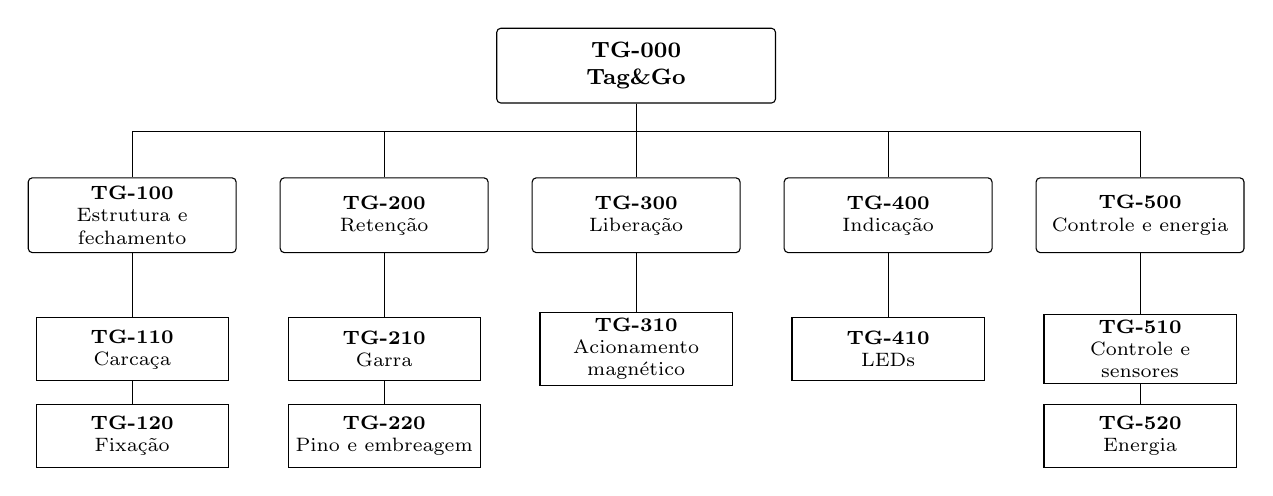
\begin{tikzpicture}[
        font=\scriptsize,
        caixa/.style={draw, rounded corners=1.5pt, align=center, text width=2.5cm, minimum height=0.95cm, inner sep=2pt},
        sub/.style={draw, align=center, text width=2.3cm, minimum height=0.8cm, inner sep=2pt}]
        \node[caixa, text width=3.4cm, font=\footnotesize\bfseries] (p) at (6.4,0) {TG-000\\Tag\&Go};
        \foreach \x/\cod/\nome in {
            0/TG-100/Estrutura e fechamento,
            3.2/TG-200/Retenção,
            6.4/TG-300/Liberação,
            9.6/TG-400/Indicação,
            12.8/TG-500/Controle e energia}{
            \node[caixa] (s\cod) at (\x,-1.9) {\textbf{\cod}\\\nome};
            \draw (p.south) -- ++(0,-0.35) -| (s\cod.north);
        }
        \foreach \x/\y/\cod/\nome in {
            0/-3.6/TG-110/Carcaça,
            0/-4.7/TG-120/Fixação,
            3.2/-3.6/TG-210/Garra,
            3.2/-4.7/TG-220/Pino e embreagem,
            6.4/-3.6/TG-310/Acionamento magnético,
            9.6/-3.6/TG-410/LEDs,
            12.8/-3.6/TG-510/Controle e sensores,
            12.8/-4.7/TG-520/Energia}{
            \node[sub] (c\cod) at (\x,\y) {\textbf{\cod}\\\nome};
        }
        \draw (sTG-100.south) -- (cTG-110.north);
        \draw (cTG-110.south) -- (cTG-120.north);
        \draw (sTG-200.south) -- (cTG-210.north);
        \draw (cTG-210.south) -- (cTG-220.north);
        \draw (sTG-300.south) -- (cTG-310.north);
        \draw (sTG-400.south) -- (cTG-410.north);
        \draw (sTG-500.south) -- (cTG-510.north);
        \draw (cTG-510.south) -- (cTG-520.north);
    \end{tikzpicture}
    \source{Elaborado pelos autores (2026).}
\end{figure}

A função de cada sistema é a seguinte.

\begin{itemize}
    \item \textbf{Estrutura e fechamento (TG-100).} Abriga e posiciona os demais sistemas e impede o acesso ao mecanismo. Inclui o suporte que mantém a embreagem e o microatuador à distância de projeto, e a tampa, que leva o código 2D gravado.
    \item \textbf{Retenção (TG-200).} Prende o dispositivo à peça. A garra fecha sobre a borda da roupa, o pino fixado nela atravessa o tecido, e a embreagem de esferas impede o recuo do pino sem consumir energia.
    \item \textbf{Liberação (TG-300).} Encerra a retenção. O microatuador gira o braço e leva os ímãs para baixo da embreagem. O campo recolhe o carretel, o pino sai, e a mola abre a garra.
    \item \textbf{Indicação (TG-400).} Os LEDs informam o estado do dispositivo: travado, em recarga e liberado.
    \item \textbf{Controle e energia (TG-500).} A placa de controle se comunica com o servidor, recebe a ordem de liberação e comanda o microatuador e os LEDs. As chaves informam se a garra está fechada e se o dispositivo está na base de recarga. A célula alimenta o conjunto e é recarregada pela bobina de indução.
\end{itemize}

\subsection{Lista estruturada de componentes}
\label{subsec:estrut_lista}

A Tabela~\ref{tab:estrut_lista} apresenta a estrutura completa. A coluna de nível indica a posição do item na árvore, e a coluna de balão indica o número do item no desenho de conjunto (Figura~\ref{fig:conj_desenho}).

\begingroup
\footnotesize
\renewcommand{\arraystretch}{1.25}
\begin{longtable}{@{}c l >{\RaggedRight\arraybackslash}p{4.6cm} c c c >{\RaggedRight\arraybackslash}p{4.4cm}@{}}
    \caption{Estrutura do produto Tag\&Go}\label{tab:estrut_lista}\\
    \toprule
    \textbf{Nível} & \textbf{Código} & \textbf{Item} & \textbf{Qtd.} & \textbf{Origem} & \textbf{Balão} & \textbf{Observação} \\
    \midrule
    \endfirsthead
    \toprule
    \textbf{Nível} & \textbf{Código} & \textbf{Item} & \textbf{Qtd.} & \textbf{Origem} & \textbf{Balão} & \textbf{Observação} \\
    \midrule
    \endhead
    \bottomrule
    \endfoot
    0 & TG-000 & \textbf{Tag\&Go} & 1 & F & -- & Produto acabado \\
    \midrule
    1 & TG-100 & \textbf{Estrutura e fechamento} & 1 & F & -- & \\
    2 & TG-110 & \hspace{0.3cm}Carcaça & 1 & F & -- & \\
    3 & TG-111 & \hspace{0.6cm}Base da carcaça & 1 & F & 1 & Fundo de 1,5 mm sobre a bobina \\
    3 & TG-112 & \hspace{0.6cm}Tampa & 1 & F & 2 & Com o código 2D gravado, o furo do pino e os furos dos LEDs \\
    3 & TG-113 & \hspace{0.6cm}Suporte do mecanismo & 1 & F & 9 & Recebe a embreagem e o microatuador \\
    2 & TG-120 & \hspace{0.3cm}Fixação & 1 & C & -- & \\
    3 & TG-121 & \hspace{0.6cm}Parafuso da tampa & 4 & C & -- & Permite retirar a célula no descarte \\
    \midrule
    1 & TG-200 & \textbf{Retenção} & 1 & F & -- & \\
    2 & TG-210 & \hspace{0.3cm}Garra & 1 & F & -- & \\
    3 & TG-211 & \hspace{0.6cm}Corpo da garra & 1 & F & 3 & Com dentes na face que toca o tecido \\
    3 & TG-212 & \hspace{0.6cm}Eixo da articulação & 1 & C & -- & Pino padronizado \\
    3 & TG-213 & \hspace{0.6cm}Mola de abertura & 1 & C & -- & Abre a garra quando o pino é liberado \\
    3 & TG-214 & \hspace{0.6cm}Revestimento de elastômero & 1 & C & -- & Aumenta o atrito com o tecido \\
    2 & TG-220 & \hspace{0.3cm}Pino e embreagem & 1 & C & -- & \\
    3 & TG-221 & \hspace{0.6cm}Pino & 1 & C & 4 & Fixado ao corpo da garra \\
    3 & TG-222 & \hspace{0.6cm}Embreagem de esferas & 1 & C & 5 & Comprada montada: copo, esferas, carretel e mola \\
    \midrule
    1 & TG-300 & \textbf{Liberação} & 1 & F & -- & \\
    2 & TG-310 & \hspace{0.3cm}Acionamento magnético & 1 & F & -- & \\
    3 & TG-311 & \hspace{0.6cm}Microatuador rotativo & 1 & C & 8 & Curso de 90$^\circ$ \\
    3 & TG-312 & \hspace{0.6cm}Braço dos ímãs & 1 & F & 7 & Raio de 16 mm \\
    3 & TG-313 & \hspace{0.6cm}Ímã de neodímio & 3 & C & 6 & $\varnothing$ 10 $\times$ 4 mm, empilhados \\
    3 & TG-314 & \hspace{0.6cm}Parafuso do braço & 1 & C & -- & Prende o braço ao eixo do microatuador \\
    \midrule
    1 & TG-400 & \textbf{Indicação} & 1 & C & -- & \\
    2 & TG-410 & \hspace{0.3cm}LEDs & 1 & C & -- & \\
    3 & TG-411 & \hspace{0.6cm}LED & 3 & C & 10 & Vermelho, amarelo e verde \\
    \midrule
    1 & TG-500 & \textbf{Controle e energia} & 1 & C & -- & \\
    2 & TG-510 & \hspace{0.3cm}Controle e sensores & 1 & C & -- & \\
    3 & TG-511 & \hspace{0.6cm}Placa de controle montada & 1 & C & 11 & Comprada montada, sob especificação do projeto. Inclui o rádio \\
    3 & TG-512 & \hspace{0.6cm}Chave da garra & 1 & C & 14 & Detecta a garra fechada \\
    3 & TG-513 & \hspace{0.6cm}Chave da base & 1 & C & 15 & Detecta a base de recarga \\
    2 & TG-520 & \hspace{0.3cm}Energia & 1 & C & -- & \\
    3 & TG-521 & \hspace{0.6cm}Célula recarregável & 1 & C & 12 & \\
    3 & TG-522 & \hspace{0.6cm}Bobina de indução & 1 & C & 13 & Receptora \\
\end{longtable}
\endgroup
% \source usa \caption*, que não funciona fora de ambiente flutuante; por isso a fonte da longtable vai como texto.
\begin{center}
    \vspace{-0.6cm}
    \footnotesize Fonte: Elaborado pelos autores (2026). F: fabricado sob desenho do projeto. C: comprado.
\end{center}

\subsection{Leitura da estrutura}
\label{subsec:estrut_leitura}

A estrutura tem 20 componentes distintos no nível 3, que somam 27 peças por dispositivo. Cinco componentes são fabricados sob desenho: a base, a tampa, o suporte do mecanismo, o corpo da garra e o braço dos ímãs. Os outros 15 são comprados.

A proporção alta de itens comprados é uma decisão de projeto. A embreagem de esferas é o componente do qual depende a segurança da retenção, e comprá-la pronta aproveita um item já fabricado em grande volume para as etiquetas rígidas. As cinco peças fabricadas concentram o que é próprio do Tag\&Go: a geometria que posiciona o ímã em relação à embreagem e a forma que prende a roupa.

Em relação à versão com tela, avaliada no modelo digital, a estrutura perdeu um sistema e dois componentes, a tela e o botão. As quantidades seguem o modelo digital e serão revistas no projeto detalhado.
